% !TEX root = ./notes.tex
\chapter{Neutron Stars}

\section{Cooling neutron stars}\label{s.cooling-neutron-stars}
First, let's get some estimates of the neutron star.  A solar mass has of order $10^{57}$ nucleons.  If we pack those nucleons so that the mean spacing is $\approx 1\nsp\fermi$, then the radius of our object is $\sim 10^{19}\nsp\fermi\sim 10\nsp\km$.  The current best observational constraints put the radius at around 12\nsp\km.  Observed masses (from radio pulsars in binaries) range from around 1.1\nsp\Msun\ up to 1.97\nsp\Msun.

Although the matter in the core of a neutron star is not an ideal gas, we'll start by ignoring the nuclear force and imagining that the core consists of cold  neutrons, proton, and electrons in a charge-neutral plasma that is in $\beta$-equilibrium. This translates into three conditions:
\begin{enumerate}
\item\label{cold-neutron-star} Cold: The chemical potentials are just the Fermi energies, $\mu = E_{\mathrm{F}}$, with
\begin{eqnarray}
	E_{\mathrm{F}} &=& \frac{\hbar^{2}}{2m}\left(3\pi^{2}n\right)^{2/3},\qquad\textrm{non-relativistic}\\
	E_{\mathrm{F}} &=& \hbar c\left(3\pi^{2}n\right)^{1/3},\qquad\textrm{relativistic}.
\end{eqnarray}
\item\label{charge-neutral-star} Charge-neutral: $n_{e} = n_{p}$.
\item\label{beta-equil-star} Beta-equilibrium: The reaction $\nt\leftrightarrow \pt+e$ is in equilibrium, so 
$ \mu_{n} = \mu_{p}+\mu_{e} - Q$,
where $Q = (m_{n}-m_{p}-m_{e})c^{2} = 0.782\nsp\MeV$.
\end{enumerate}

The proton fraction (and therefore the electron fraction) is indeed quite small at low density (near nuclear saturation density) where the protons and neutrons are non-relativistic (exercise).  The proton-to-neutron ratio increases with density.  The reactions to maintain $\beta$-equilibrium emit a neutrino: $\nt \to \pt + e + \bar{nu}_{e}$ and $\pt + e \to \nt + \nu_{e}$.  After the first few seconds, the temperatures are well below $10\nsp\MeV$, and the neutrino mean free path is larger than the stellar radius.  Since the star is degenerate, the source of free energy for the neutrinos cannot come from contraction, and the neutron star must cool.

These reactions (named \emph{Urca} reactions by Gamow) would indeed cause the neutron star to cool exceedingly rapidly, but there is one hitch: the reactions are blocked (exercise).  As a result, neutrino emission proceeds via the modified Urca reactions:
\begin{eqnarray}
\nt+\nt &\to& \nt + \pt + e + \bar{\nu}_{e}\\
\nt + \pt + e &\to& \nt + \nt + \nu_{e}.
\end{eqnarray}

\section{Accreting neutron stars}

\subsection{Basics of Mass Transfer}\label{s.mass-transfer}

Suppose we have two objects orbiting a common center of mass.  By convention, the more massive object is known as the \emph{primary} and will be denoted by a subscript ``1''; the less massive object is the \emph{secondary} and is denoted by a subscript ``2''.  From Kepler's law, the orbital separation is
\begin{equation}\label{e.orbital-separation}
	a^{3} = G(M_{1}+M_{2}) \left(\frac{P}{2\pi}\right)^{2}, 
\end{equation}
with a numerical value $a = 0.51\nsp R_{\sun} (m_{1}+m_{2})^{1/3} (P/\hour)^{2/3}$, where we've scaled our masses to solar values, $m = M/\Msun$.

In a co-rotating frame, there is an equipotential surface with a saddle point, the \emph{inner Lagrange point}, between the two stars.  This surface forms two lobes, the \emph{Roche} lobes, that meet at this point. See the crude sketch in Figure~\ref{f.roche}.
Although the Roche lobes are not spherical, we can define the radius of an equivalent spherical volume; for the secondary, this is
\begin{equation}\label{e.r2-roche}
\frac{R_{2}}{a} \approx 0.462 \left(\frac{M_{2}}{M_{1} + M_{2}}\right)^{1/3}.
\end{equation}
As an aside, equations~(\ref{e.r2-roche}) and (\ref{e.orbital-separation}) imply that the average density of the secondary, if it fills its Roche lobe, is
\[
	\bar{\rho} = \frac{3M_{2}}{4\pi R_{2}^{3}} \approx 111\nsp\grampercc\left(\frac{\hour}{P}\right)^{2}.
\]
and does not depend explicitly on the masses of the two stars.

\begin{figure}[htbp]
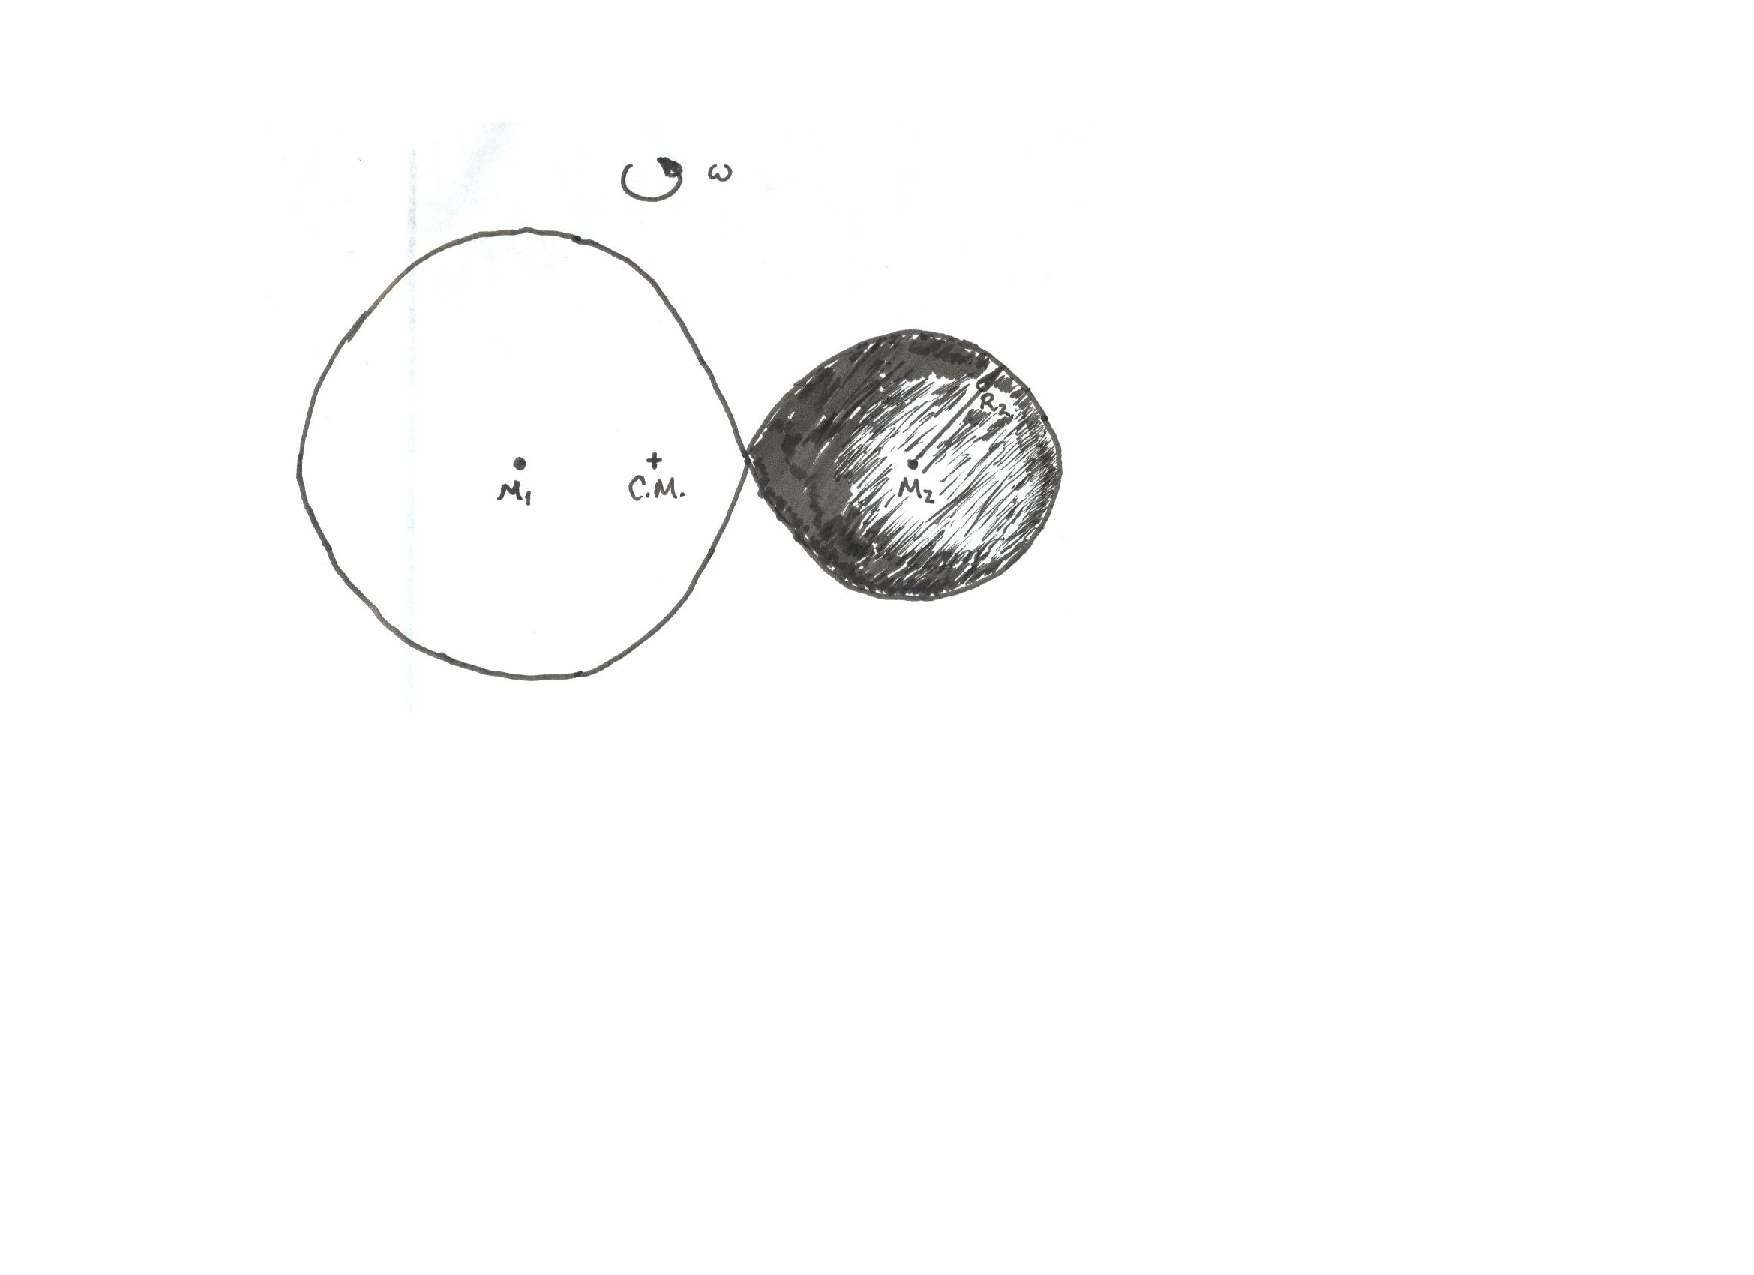
\includegraphics{Figures/roche-sketch}
\caption[Schematic of Roche lobes]{\label{f.roche} Sketch of the Roche lobes. Here the secondary, $M_{2}$, is depicted as filling its lobe.}
\end{figure}

If matter is transferred from $M_{2}$ to $M_{1}$ how does the system respond?  Let's first write down the angular momentum of the system,
\begin{equation}\label{e.roche-J}
J = (M_{1}a_{1}^{2} + M_{2}a_{2}^{2}) \omega = M_{1}M_{2}\left(\frac{Ga}{M_{1}+M_{2}}\right)^{1/2}.
\end{equation}
Here we've used equation~(\ref{e.orbital-separation}) and the relations $a_{1} = aM_{2}/(M_{1}+M_{2})$, $a_{2} = aM_{1}/(M_{1}+M_{2})$.  Let's make the assumption that no mass is lost from the system and that the mass transfer $\dot{M}$ is from $M_{2}$ to $M_{1}$:
\begin{eqnarray*}
\dot{M}_{1} + \dot{M}_{2} &=& 0;\\
\dot{M}_{2} = -\dot{M} &<& 0.
\end{eqnarray*}
Taking the logarithm of equation~(\ref{e.roche-J}) and differentiating, we then obtain
\begin{equation}\label{e.roche-adot}
\frac{\dot{a}}{a} = 2\frac{\dot{J}}{J}  + 2 \left(\frac{\dot{M}}{M_{2}}\right) \left(1-\frac{M_{2}}{M_{1}}\right).
\end{equation}
We see explicitly that for $M_{2}< M_{1}$, the response of mass transfer is to increase the orbital separation $a$ if there is no external torque on the system.

What about the size of the lobe that the secondary inhabits?  There are two countervailing tendencies: $a$ increases, which acts to increase $R_{2}$, but $M_{2}$ decreases, which acts to decrease $R_{2}$.  Taking the logarithm of eq.~(\ref{e.r2-roche}),
\begin{equation}\label{e.r2dot}
\frac{\dot{R}_{2}}{R_{2}} = \frac{\dot{a}}{a} + \frac{1}{3}\frac{\dot{M}_{2}}{M_{2}} = 2\frac{\dot{J}}{J} + 2\frac{\dot{M}}{M_{2}} \left(\frac{5}{6} - \frac{M_{2}}{M_{1}}\right).
\end{equation}
Hence for $M_{2} < (5/6) M_{1}$, the volume of the secondary's Roche lobe increases; if the secondary doesn't expand in response to mass loss and there are no external torques, then the secondary will lose contact with the inner Lagrange point and mass transfer will cease.  Alternatively, if $M_{2} > (5/6) M_{1}$, then the Roche lobe will clamp down on the secondary; this tends to drive the mass transfer at an even greater rate, and the process is unstable.

In general, there are three physical mechanisms for driving mass transfer.
\begin{description}
\item[Gravitational radiation] For $P \lesssim 2\nsp\hour$, gravitational radiation from the orbit produces a negative torque on the system:
\begin{equation}\label{e.GR-torque}
\frac{\dot{J}}{J} = -\frac{32}{5}\frac{G^{3}}{c^{5}}\frac{M_{1}M_{2}(M_{1}+M_{2})}{a^{4}}.
\end{equation}
Note that for this short of an orbital period, the binary consists of two degenerate stars (e.g., WD-WD, NS-WD).
\item[Magnetic braking] At somewhat longer periods $P \lesssim \unit{1}{d}$, the companion can be a main sequence star that has a tidally locked rotation period.  Main-sequence stars have winds, and these winds carry angular momentum.  Because of the tidal locking, this also introduces a negative torque on the system.
\item[Evolution of the secondary] For wider binary orbits, the secondary star can make contact with the Roche lobe as it becomes a giant star.
\end{description}
Finally, if the secondary is sufficiently evolved, it may have a strong enough wind that accretion can still occur, even if the orbit is so wide that the secondary doesn't fill its Roche lobe.

Matter that crosses the inner Lagrange point will find itself in orbit about the primary.  The material still has enough angular momentum that it won't fall directly onto the primary, and so an \emph{accretion disk} will form. In order for the matter to accrete, there must be enough friction in the disk so that the gravitational energy can be radiated away and angular momentum transported outward.

\subsection{The Eddington Limit}

There is a characteristic luminosity at which the pressure from radiation balances the gravitational force.  This tends to act as a limit to accretion.  To derive this limit, known as the \emph{Eddington luminosity}, consider a spherically symmetric shell of matter.  Radiation enters the shell and scatters isotropically (Thomson scatters) from electrons.  The momentum flux (momentum per unit time per unit area) entering the shell is just
\[
	\bvec{P} = \frac{1}{c}\frac{L}{4\pi r^{2}} \bvec{e}_{r}.
\]
Here $L$ is the luminosity and $r$ is the radius of the shell.  Since the scattering is presumed isotropic, the rate at which the fluid element's momentum changes (the impulse imparted to it by the radiation) is just
\[
	\frac{\dif \bvec{p}}{\dif t} = \bvec{P}\sigma_{\mathrm{Th}} n_{e},
\]
where $\sigma_{\mathrm{Th}}$ is the cross-section for Thomson scattering.  Since $\dif\bvec{p}/\dif t$ is just a force per unit volume, we can balance it with the gravitational force per unit volume,
\[
\bvec{f}_{g} = -\frac{GM \langle A\rangle \mb n_{\mathrm{ion}}}{r^{2}}\bvec{e}_{r},
\]
and solve for $L$ to obtain
\begin{equation}\label{e.Ledd}
L_{\mathrm{Edd}} = \frac{4\pi GM c}{(\sigma_{\mathrm{Th}}/\mb)Y_{e}}.
\end{equation}
Here I have used $n_{e} = \langle Z\rangle n_{\mathrm{ion}}$ and $Y_{e} = \langle Z\rangle/\langle A\rangle$.
Note that $L_{\mathrm{Edd}}$ is independent of distance from the star.  Numerically,
\[ L_{\mathrm{Edd}} = 1.3\ee{38}\nsp\ergspersecond \left(\frac{M}{\Msun}\right)Y_{e}^{-1} 
	= 3.2\ee{4}\Lsun \left(\frac{M}{\Msun}\right) Y_{e}^{-1}.
\]
We can now look at what the luminosity supplied by accretion is.  First there is the just the gravitational energy release.  The gravitational release, per nucleon, is
\[ \frac{GM\mb}{R} =  \left\{\begin{array}{lr}0.069\nsp\MeV & \textrm{WD with $R=2\ee{9}\nsp\cm$}
	 \\ 138\nsp\MeV & \textrm{NS with $R = 10^{6}\nsp\cm$}\end{array}\right.
\]
In both cases we used $M = 1\nsp\Msun$.  For hydrogen-rich accretion onto a white dwarf, steady nuclear burning (assuming it exists!) will dwarf the luminosity from accretion. The situation is reversed for a neutron star, for which the energy from nuclear burning is a perturbation to the large release of gravitational binding energy.

We can compute the accretion rate at which the luminosity supplied by either nuclear burning or release of gravitational binding energy would equal the Eddington value:
\[
\dot{M}_{\mathrm{Edd}} = \left\{\begin{array}{lr}
	\frac{4\pi GM c}{Q(\sigma_{\mathrm{Th}}/\mb)Y_{e}}  & \textrm{nuclear,}\nsp L = \dot{M}Q \\
	\frac{4\pi R c}{(\sigma_{\mathrm{Th}}/\mb)Y_{e}} & \textrm{gravitational,}\nsp L= \frac{GM\dot{M}}{R}
\end{array}\right. .
\]
For nuclear burning, taking $M = 1\nsp\Msun$, $Q = 6\ee{18}\nsp\ergspergram$ (hydrogen burning), and $Y_{e} = 1$ gives $\dot{M}_{\mathrm{Edd}} = 3.3\ee{-7}\nsp\Msun\usp\yr^{-1}$.  For gravitational power, taking $R = 10^{6}\nsp\cm$ and $Y_{e} = 1$ gives $\dot{M}_{\mathrm{Edd}} = 1.5\ee{-8}\nsp\Msun\usp\yr^{-1}$.  Observed systems do in fact have inferred mass transfer rates that are typically less than these values.

\subsection[Accreting Neutron Star Envelopes]{Structure of an Accreting Neutron Star Envelope}

This section is similar in spirit to lectures \citep{bildsten:thermonuclear} given at a NATO Advanced Studies Institute.

As a worked example, we shall consider the thermonuclear stability of hydrogen/helium accretion onto a neutron star.  For accretion from a disk, the luminosity (cf.\ problem~\ref{p.disk-L}) is $GM\dot{M}/(2R)$.  The remainder of the gravitational binding energy is liberated at a boundary layer where the disk becomes incorporated into the star.  Setting this equal to thermal emission gives an effective temperature
\[
	\Teff = \left(\frac{GM\dot{M}}{2R\ssb\mathcal{A}}\right)^{1/4} = 10^{7}\nsp\K \left(\frac{M}{1.4\nsp\Msun}\frac{10^{6}\nsp\cm}{R}\frac{10^{13}\nsp\cm^{2}}{\mathcal{A}}\frac{\dot{M}}{10^{-9}\nsp\Msun\usp\yr^{-1}}\right)^{1/4}
\]
Here we have scaled the emitting area to $\mathcal{A}$ rather than presuming it is emitted from the entire surface. This effective temperature is, in energy units, $\kB \Teff\approx \nsp\keV$, which is in the X-ray region of the spectrum.  

The gravitational acceleration at the neutron star surface is
\[
	g = \frac{GM}{R^{2}}\left(1-\frac{2GM}{Rc^{2}}\right)^{-1/2}\approx 2.4\ee{14}\nsp\cm\usp\second^{-2}
\]
for a neutron star with $M = 1.4\nsp\Msun$, $R = 10^{6}\nsp\cm$.  The factor in parenthesis is a correction due to general relativity. The redshift, i.e., the fractional increase in wavelength of a photon emitted from the surface to a distant observer, is $\Delta \lambda/\lambda = [1-2GM/(Rc^{2}]^{-1/2} - 1 \approx 0.3$.   Given the surface gravity and the temperature, we can estimate the pressure scale height,
\[
 H = \frac{P}{\rho g} = \frac{\kB T}{\mu\mb g} \approx 5\nsp\cm.
\]
Because $H/R\ll 1$, we can make two simplifying assumptions: first, we can treat our atmosphere in planar geometry, and second we can boost to a local frame and perform our calculations in Euclidian space-time.

In a planar geometry, there is a simple relation between the time since a fluid element was deposited and its local pressure. If we assume that accreted matter spreads uniformly over the surface, than every square centimeter sees mass being added at a rate $\dot{m} = \dot{M}/(4\pi R^{2})$.  Thus after a time $t$ a fluid element will find itself under a column with a mass per unit area $\dot{m}\times t = \int_{z}^{\infty}\rho\usp\dif z$. Using hydrostatic equilibrium, we can transform $\rho\usp\dif z = -\dif P/g$, so that
\[
P(t) = \dot{m}tg.
\]
Here $t$ is the time since the fluid element was accreted.  At an accretion rate of $\dot{M} = 10^{-9}\nsp\Msun\usp\yr^{-1}$ onto a $10\nsp\km$ neutron star, the pressure reached when the hydrogen is half-consumed is $P = 1.8\ee{22}\nsp\dyne\usp\cm^{-2}$.  The quantity $y\equiv \int_{z}^{\infty}\rho\usp\dif z$ is known as the \emph{column density}.

\subsubsection{H burning}

Let's consider the accretion of a (roughly solar) mixture of \hydrogen, \helium, and \carbon, with mass fractions $X_{\mathrm{H}}:X_{\mathrm{He}}:X_{\mathrm{CNO}} = 0.70:0.28:0.02$. At temperatures $> 10^{7}\nsp\K$, the \hydrogen\ is consumed via the hot CNO cycle,
\[
	\carbon(\pt,\gamma)\nitrogen[13](\pt,\gamma)\oxygen[14](\beta^{+}\nu)\nitrogen[14](\pt,\gamma) \oxygen[15](\beta^{+}\nu)\nitrogen[15](\pt,\alpha)\carbon.
\]
The two slowest  reactions are the decays of \oxygen[14] ($\tau_{1/2} = 71\nsp\second$) and \oxygen[15] ($\tau_{1/2} = 122\nsp\second$). As a result, the cycle is independent of temperature and thermally stable.
How long would it take to consume all of the hydrogen?  For each CNO nucleus, there are
\[ n_{\mathrm{H}}/n_{\mathrm{CNO}} = \frac{0.7}{0.02/12} = 420 \]
hydrogen nuclei, and each trip around the cycle consumes 4 hydrogen nuclei. As a result, it take 105 trips around the CNO cycle to deplete the hydrogen.  The time to complete one cycle is $(71\nsp\second + 122\nsp\second) /\ln 2 = 278\nsp\second$, so the time to deplete all of the hydrogen is $2.92\ee{4}\nsp\second$---about $1/3$ of a day.

To get the temperature structure of the accreted envelope, we use the flux equation, eq.~(\ref{e.flux}),
\begin{equation}\label{e.mod-flux}
F = -\frac{1}{3}\frac{c}{\rho\kappa}\frac{\dif aT^{4}}{\dif r}.
\end{equation}
We can again transform $\rho\usp\dif r = -\dif P/g$; moreover, if all of the heat released by fusing hydrogen to helium comes out (and assuming there is no other source of heat in the neutron star interior), the flux will just be $QX_{\mathrm{H}}\dot{m}$ and will be constant. Integrating eq.~(\ref{e.mod-flux}) and neglecting $\Teff$ and $P(\textrm{photosphere})$ gives us a relation for the temperature,
\[	T^{4} = \frac{3\kappa Fy}{ac}. \]
For the parameters we are considering, $F = QX_{\mathrm{H}}\dot{m} = 2.1\ee{22}\nsp\ergspersecond\usp\cm^{-2}$, and the temperature at the depth where the H is half-consumed is $T = 2.9\ee{8}\nsp\K$.

The cooling timescale for this atmosphere is
\[ t_{\mathrm{th}} = \frac{yC_{P} T}{F} \approx 208\nsp\second \times \frac{y_{8} T_{8}}{F_{22}} \]
Here we are using the shorthand notation, $y_{8}\equiv y/(10^{8}\nsp\columnunit)$, and similarly for $T_{8}$, $F_{22}$, and so on.
The thermal timescale can be compared to the accretion timescale,
\[ t_{\mathrm{ac}} = \frac{y}{\dot{m}} = 10^{4}\nsp\second\times y_{8}\dot{m}_{4}^{-1}.
\]
Because $t_{\mathrm{th}}\ll t_{\mathrm{ac}}$, the compression is slow and far from adiabatic.

\subsubsection{He ignition}

As the fluid element is compressed and heated, the lifetime of a \helium\ nucleus against the triple-alpha reaction becomes shorter than the accretion timescale and helium ignites.  If protons are present, then there will be additional heating from $\carbon(\pt,\gamma)$.  The triple-alpha reaction is strongly temperature sensitive and therefore is susceptible to an thermal instability.

To evaluate the thermal instability, we approximate the cooling rate as
\begin{equation}\label{e.cooling-rate-approx}
\epsilon_{\mathrm{cool}} \approx \frac{C_{P}T}{t_{\mathrm{th}}} = \frac{ac T^{4}}{3\kappa y^{2}}
\end{equation}
and compare it against the heating rate from the triple-alpha reaction, $\epsilon_{3\alpha}$. We then apply a constant-pressure thermal perturbation about the steady-state, $\epsilon_{\mathrm{cool}} = \epsilon_{3\alpha}$; upon expanding this equation we arrive at a condition for instability:
\begin{equation}\label{e.3a-instability}
\left.\frac{\partial\ln\epsilon_{3\alpha}}{\partial\ln T}\right|_{y} > \left.\frac{\partial\ln\epsilon_{\mathrm{cool}}}{\partial\ln T}\right|_{y}.
\end{equation}
The triple-alpha heating rate is 
\[
	\epsilon_{3\alpha} \approx (5.3\ee{21}\nsp\ergspersecond\usp\gram^{-1}) \times \frac{\rho_{5}^{2}X_{\mathrm{He}}^{3}}{T_{8}^{3}}\exp\left(-\frac{44}{T_{8}}\right).
\]
If we ignore the variation in density, $\rho = 10^{5}\nsp\grampercc \times \rho_{5}$, with temperature, then equation~(\ref{e.3a-instability} becomes
\begin{equation}\label{e.3a-instability-temperature}
\frac{44}{T_{8}} - 3 > 4;
\end{equation}
put another way, a thermal instability is expected to occur if $T < 6.3\ee{8}\nsp\K$ at the depth where helium is consumed.  This is satisfied for all $\dot{m}< \dot{m}_{\mathrm{Edd}}$.

The remaining question is the depth at which the triple-alpha reaction ignites.  For a rapidly accreting neutron star, the flux is greater, and therefore the envelope has a steeper temperature gradient. Consult \citet{bildsten:thermonuclear} for details; roughly, for $\dot{m} \gtrsim 0.1\dot{m}_{\mathrm{Edd}}$, the helium ignition occurs in a bath of protons, so that an rp-process ensues. The consumption of hydrogen releases more energy and requires waiting for $\beta+$-decays, this tends to produce a longer-lasting X-ray burst that is more energetic, for the amount of fuel accreted.    At lower accretion rates, the hot CNO cycle consumes all of the available hydrogen before the helium ignites; as a result, the burst is more rapid, and less energetic for the amount of matter accreted.  Note that the pure helium burst may still release a greater total amount of energy if it ignites at a greater depth, i.e., if the amount of matter accumulated between bursts is greater.

\section{Exercises}
\begin{enumerate}
\item Find the equilibrium proton-to-neutron ratio, $x = n_{p}/n_{n}$.  The electrons, being light, are always relativistic.  Show that $x$ is indeed vary small but increases with density in the limit of both neutrons and protons being non-relativistic. In the opposite limit, all three particles relativistic, show that $x\to 1/8$.  \emph{Hint:} neglect the electron mass and the difference between the neutron and proton masses; use the values $\hbar c = 197.327\nsp\MeV\usp\fermi$ and $m_{n}c^{2} = 939.565\nsp\MeV$, and scale the neutron density $n_{n}$ to the nuclear saturation density $n_{0}= 0.16\nsp\fermi^{-3}$.

\item Show that the reactions
\begin{eqnarray*}
\nt &\to& \pt + e + \bar{\nu}_{e}\\
\pt +e &\to& \nt + \nu_{e}
\end{eqnarray*}
cannot simultaneously conserve momentum and energy if the $\nt$, $\pt$, and $e$ are on their respective Fermi surfaces.  Take the neutrons and protons to be non-relativistic, the electrons to be relativistic, and presume that the plasma is charge-neutral and in $\beta$-equilibrium. Neglect the electron rest mass and the difference between the neutron and proton rest masses.  Recall that the momentum of a particle on its Fermi surface is $p_{\mathrm{F}} = \hbar(3\pi^{2} n)^{1/3}$, so that $E_{\mathrm{F}} = p_{\mathrm{F}}^{2}/(2m)$ if non-relativistic and $E_{\mathrm{F}} = p_{\mathrm{F}}c$ if relativistic.

\item Suppose our binary consists of two white dwarfs with a short orbital period, less than 2 hours, so that gravitational radiation produces a torque on the system according to eq.~(\ref{e.GR-torque}).  Because the secondary is also degenerate, its radius depends on mass as
\[ R_{2} = K \left(\frac{M_{2}}{\Msun}\right)^{-1/3}, \]
where $K \approx 2\ee{9}\nsp\cm$.
\begin{enumerate}
\item Show that if the secondary just fills its Roche lobe, then $M_{2} \propto P^{-1}$ and find $M_{2}$ if $P = 1\nsp\hour$.
\item Show that
\[ \frac{\dot{M}}{M_{2}} = - \frac{\dot{J}/J}{2/3 - M_{2}/M_{1}} \]
\item Using the above relations and eq.~(\ref{e.GR-torque}), find $\dot{M}$ if $M_{1} = 1\nsp\Msun$. Scale the orbital period to units of 1 hour.
\end{enumerate}

\item Suppose we have a $1.6\nsp\Msun$ neutron star and a $0.8\nsp\Msun$ companion.  The companion is evolved and has an effective temperature $\Teff = 3000\nsp\K$.  We'll assume that $\Teff$ is fixed.  On the giant branch, the luminosity is powered by hydrogen shell burning, the ashes of which are added to the core (i.e., the core mass $M_{c}$ increases due to hydrogen burning).  The energy released, per gram of hydrogen consumed, is $Q = 6\ee{18}\nsp\ergs\usp\gram^{-1}$. For such an evolved giant the luminosity depends mainly on the core mass $M_{c}$ and may be approximated as \citep{Ritter1999Analytical-solu}
\[
	\frac{L}{\Lsun} = 10^{6.3}\left(\frac{M_{c}}{\Msun}\right)^{8}.
\]
For this system, find the orbital period $P$ and the mass transfer rate $\dot{M}$ (in units of solar masses per year) if the secondary has a core mass $M_{c} = 0.2\nsp\Msun$. 

\item \label{p.disk-L} Consider a star surrounded by an accretion disk of matter.  In the disk, which consists of ionized gas, a fluid element gradually spirals inward, so that at each point in the disk, it is approximately in a circular orbit.  Show that under these conditions, the energy radiated, per unit mass, by the fluid element over its lifetime in the disk is $GM/(2R)$.

\end{enumerate}
